%%%%%%%%%%%%%%%%%%%%%%%%%%%%%%%%%%%%%%%%%%%%%%%%%%%%%%%%%%%%%%%%%%%%%
%
%  This is a sample LaTeX input file for your contribution to ICTT25.
%  Modified by from the ICTT24 template by Vittorio Romano, UNICT, who
%  got ICTT23 template from Jim Warsa, LANL, who got the MC2013
%  template from R.C. Martineau at INL from A. Sood at LANL, from
%  J. Wagner ORNL who obtained the original class file by Jim Warsa,
%  LANL, 16 July 2002}
%
%  Please use it as a template for your full paper 
%    Accompanying/related file(s) include: 
%       1. Document class/format file: ictt25.cls
%       2. Sample Postscript Figure:   figure.eps
%       3. A PDF file showing the desired appearance: template.pdf 
%    Direct questions about these files to: gentile1@llnl.gov
%
%    Notes: 
%
%      (1) You can make this document most easily by typing ``pdflatex
%      template.tex'' at the prompt.
%
%      (2) Different versions of LaTeX have been observed to 
%          shift the page down (as seems to be the case if your
%          latex installation has A4 paper as default), causing 
%          improper margins. If this occurs, adjust the "topmargin" 
%          value in the ictt25.cls file to achieve the proper margins. 
%
%%%%%%%%%%%%%%%%%%%%%%%%%%%%%%%%%%%%%%%%%%%%%%%%%%%%%%%%%%%%%%%%%%%%%


%%%%%%%%%%%%%%%%%%%%%%%%%%%%%%%%%%%%%%%%%%%%%%%%%%%%%%%%%%%%%%%%%%%%%

\documentclass{ictt25}
%
%  various packages that you may wish to activate for usage 
\usepackage{amsmath}
\usepackage{graphicx}
\usepackage{tabls}
\usepackage{afterpage}
\usepackage{cites}
\usepackage{epsf}

%
% Insert authors' names and short version of title in lines below
%

\newcommand{\authorHead}      % Author's names here
   {Samuel S. Olivier, Jim E. Morel}  
\newcommand{\shortTitle}      % Short title here
   {Variable Eddington Factor Method}  

\renewcommand\Authfont{\normalsize} 
\renewcommand\Affilfont{\itshape\small}

%%%%%%%%%%%%%%%%%%%%%%%%%%%%%%%%%%%%%%%%%%%%%%%%%%%%%%%%%%%%%%%%%%%%%
%
% Set title and authors here
%
%%%%%%%%%%%%%%%%%%%%%%%%%%%%%%%%%%%%%%%%%%%%%%%%%%%%%%%%%%%%%%%%%%%%%

\title{Variable Eddington Factor Method}

\author[1]{S. Olivier} 
\author[2]{J. Morel} 
\affil[1]{solivier@berkeley.edu, University of California, Berkeley}
\affil[2]{morel@tamu.edu, Texas A\&M University} 

%%%%%%%%%%%%%%%%%%%%%%%%%%%%%%%%%%%%%%%%%%%%%%%%%%%%%%%%%%%%%%%%%%%%%
%
%   BEGIN DOCUMENT
%
%%%%%%%%%%%%%%%%%%%%%%%%%%%%%%%%%%%%%%%%%%%%%%%%%%%%%%%%%%%%%%%%%%%%%

\begin{document}

\normalsize

%      Headers and Footers

\afterpage{%
\fancyhf{}%
\fancyhead[CE]{              
{\scriptsize \authorHead}}                                                
\fancyhead[CO]{               
{\scriptsize \shortTitle}}                  
\rfoot{\thepage/\totalpages{}}%

%     Change this if your installation causes the document to be shifted downward
%\setlength{\topmargin}{-20pt}
}

\pagestyle{fancy}
 
\maketitle

%
% SET RAGGED RIGHT MARGIN
%
\raggedright

%\setlength{\baselineskip}{14pt}
\normalsize

\Section{Introduction} 
\label{sec:intro}

If you are a {\LaTeX} expert you can likely define the established 
format characteristics in a more elegant manner than what is done here.  
We request that you limit the summary to two pages.
You need not have multiple sections.

\Section{Next Section} 
\label{sec:first}

This is Section~\ref{sec:first}. 
Equations, such as Eq.~\ref{equ:example-equation}, are numbered to the right of the formula.
%
\begin{equation}
\label{equ:example-equation}
\Omega \cdot \nabla \psi + \sigma_t(r) \psi(r,\Omega) = \dfrac{\sigma_s(r)}{4 \pi} \int_{4 \pi} d\Omega^{\prime} \psi(r, \Omega^{\prime}) + Q(r, \Omega)
\end{equation}

Figures, such as Fig.~\ref{fig:example-figure}, may be included using
the includegraphics command. The first example imports an eps file; you can vary
the size using the ``scale'' command:
%
\begin{figure}[!htb]
\begin{center}
%\includegraphics[scale=0.45,clip=true,viewport=42 58 709 527]{./figure.eps} 
\includegraphics[scale=0.3,clip=true]{./figure.eps} 
\begin{spacing}{1.0}
\caption{A solution to the one-dimensional slab geometry integral 
equation using 256-point Gauss-Legendre quadrature.% include label in command for correct ref count
\label{fig:example-figure}}
\end{spacing}
\end{center}
\end{figure}

The second example imports a pdf file; you can vary
the size using the ``height'' command:
%
\begin{figure}[!htb]
\begin{center}
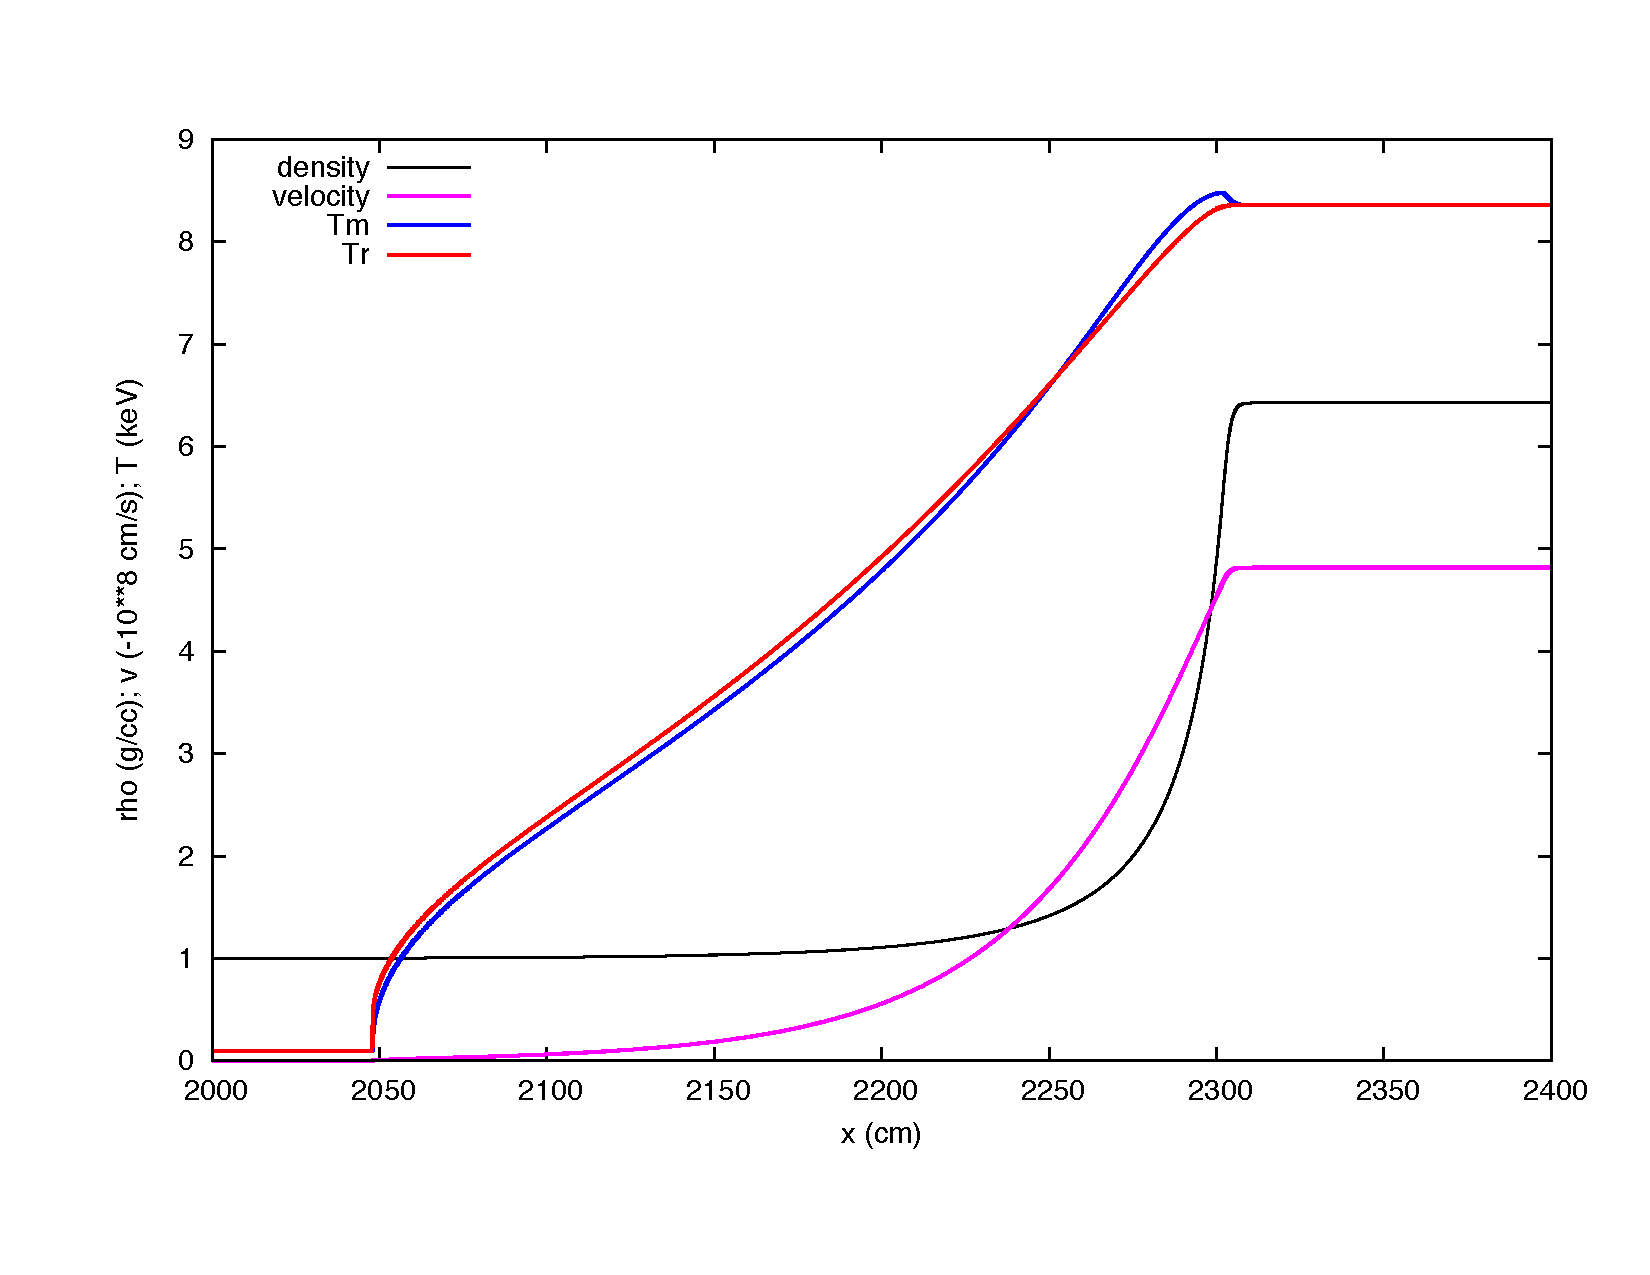
\includegraphics[height=0.3\textheight]{Mach45ICs.pdf}
\begin{spacing}{1.0}
\vspace{-15pt}
\caption{Initial values for density, velocity, and matter
  and radiation temperature for the Mach 45 radiating shock.}
\label{fig:ICs}
\end{spacing}
\end{center}
\end{figure}
%

See Table \ref{tbl:example-table} for an example of a table.  The tabls package is
recommended for improved row and column spacing.  The caption appears 
above the table by setting the caption command immediately after 
the begin table command.
%
\begin{table}[!htb]
\caption{A table example that you should format to your own tastes.% include label in command for correct ref count
\label{tbl:example-table}} 
\begin{center}
\begin{tabular}{r|ll} \hline 
 Heading  & \multicolumn{2}{c}{Columns of Numbers} \\ \hline \hline
\ 1 &  100.0 & 2.0  \\ \hline
\ 2 &  $1.0 \cdot 10^{-4}$  & 0.40 \\ \hline 
\end{tabular}
\end{center}
\end{table}

\Section{Conclusions}

A summary and conclusions might go here.

\section*{Acknowledgements}

Most of the {\LaTeX} format contained in this class file and template
were adapted by J.~Warsa (LANL) from the MC2013 conference template.

% for those who wish not to use a .bib file:

\setlength{\baselineskip}{12pt}
\begin{thebibliography}{300}
\bibitem{journal} A. Author, ``Article,'' {\it Journal Name}, vol.~1, pp. 1--199 (2013).
\bibitem{proc_paper} A. Author, ``Paper,'' {\it Proceedings of Meeting}, Location, Dates, vol.~1, pp. 5209--5314 (2013).
\bibitem{book} A. Author, {\it Book Title}, Publisher, City \& Country (2013). 
\bibitem{website} ``A Website for Everything,'' http://this.is.not.a.site/nothing (2013).
\end{thebibliography}


\end{document}
